% This file was created by matlab2tikz.
%
%The latest updates can be retrieved from
%  http://www.mathworks.com/matlabcentral/fileexchange/22022-matlab2tikz-matlab2tikz
%where you can also make suggestions and rate matlab2tikz.
%
\definecolor{mycolor1}{rgb}{0.00000,0.44700,0.74100}%
\definecolor{mycolor2}{rgb}{0.85000,0.32500,0.09800}%
%
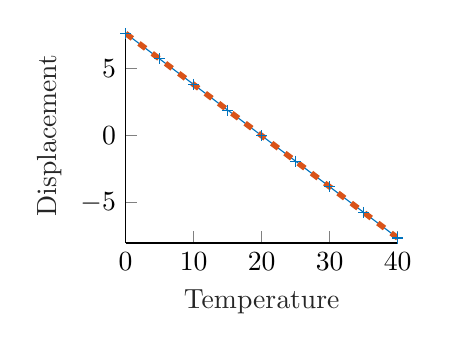
\begin{tikzpicture}

\begin{axis}[%
width=0.285\textwidth,
height=0.225\textwidth,
at={(0\textwidth,0\textwidth)},
scale only axis,
unbounded coords=jump,
xmin=0,
xmax=40,
xlabel style={font=\color{white!15!black}},
xlabel={Temperature \si{\celsius}},
ymin=-8,
ymax=8,
ylabel style={font=\color{white!15!black}},
ylabel={Displacement \si{\micro\meter}},
axis background/.style={fill=white},
axis x line*=bottom,
axis y line*=left
]
\addplot [color=mycolor1, mark=+, mark options={solid, mycolor1}, forget plot]
  table[row sep=crcr]{%
0	7.61437295767633\\
5	5.71264870995948\\
10	3.80834090012571\\
15	1.9015454140768\\
20	-0.00339751868487469\\
25	-1.90851902814607\\
30	-3.81384281695528\\
35	-5.71963254680427\\
40	-7.62575267443897\\
45	nan\\
50	nan\\
55	nan\\
60	nan\\
65	nan\\
70	nan\\
75	nan\\
80	nan\\
85	nan\\
90	nan\\
95	nan\\
100	nan\\
};
\addplot [color=mycolor2, dashed, line width=2.0pt, forget plot]
  table[row sep=crcr]{%
40	-7.62458927869706\\
0	7.61698114465458\\
};
\end{axis}
\end{tikzpicture}%